\documentclass[10pt]{article}

\usepackage[tight,hang,nooneline,raggedright,FIGTOPCAP,figbotcap,scriptsize]{subfigure}
\usepackage{colortbl}
\usepackage{color}
\usepackage{url}
\usepackage{times}
\usepackage{amsmath,amssymb,latexsym}
\usepackage{epsfig}
\usepackage{wrapfig}
\usepackage{listings}
\usepackage{multicol}
\usepackage{indentfirst} 
\usepackage{proof}
\usepackage{amsthm}
\usepackage{mathrsfs}
\usepackage{stmaryrd}
\usepackage{graphicx}
\usepackage{wrapfig}

\newtheorem{definition}{Definition}
\newcommand{\CADENA}{\textsc{Cadena}}
\newcommand{\sparkcode}[1]{{\sf {#1}}}
\newenvironment{dispcode}{\begin{center}\sf\begin{tabbing}}{\end{tabbing}\end{center}}
\newcommand{\propfont}[1]{{\sf {#1}}}

% page display
\topmargin=0in \headheight=0in \oddsidemargin=0in
\evensidemargin=0in \textwidth=6.5in \textheight=9in

\renewcommand{\topfraction}{.99}
\renewcommand{\textfraction}{.}
\renewcommand{\floatsep}{2pt}
\renewcommand{\textfloatsep}{2pt}
\renewcommand{\floatpagefraction}{.99}


\newenvironment{smallitemize}{\setlength{\topsep}{0.0 truein}
   \begin{itemize}
   \setlength{\leftmargin}{.25 truein}
   \setlength{\parsep}{0.0 truein}
   \setlength{\parskip}{0.0 truein}
   \setlength{\itemsep}{0.0 truein}}{\end{itemize}}

\newenvironment{smalldescription}{\setlength{\topsep}{0.0 truein}
   \begin{description}
   \setlength{\leftmargin}{.25 truein}
   \setlength{\parsep}{0.0 truein}
   \setlength{\parskip}{0.0 truein}
   \setlength{\itemsep}{0.0 truein}}{\end{description}}

\newenvironment{smallenumerate}{\setlength{\topsep}{0.0 truein}
   \begin{enumerate}
   \setlength{\leftmargin}{0.25 truein}
   \setlength{\parsep}{0.0 truein}
   \setlength{\parskip}{0.0 truein}
   \setlength{\itemsep}{0.0 truein}}{\end{enumerate}}

\newenvironment{flatenumerate}{\setlength{\topsep}{0.0 truein}
   \begin{enumerate}
   \setlength{\leftmargin}{0.25 truein}
   \setlength{\parsep}{0.0 truein}
   \setlength{\parskip}{0.0 truein}
   \setlength{\itemsep}{0.0 truein}}{\end{enumerate}}

\newenvironment{myitemize}[1]%
               {\begin{itemize}\setlength{\itemsep}{#1}}%
               {\end{itemize}}

\def\sqzhuge{\vspace{-14pt}}
\def\sqzlarge{\vspace{-12pt}}
\def\sqzsub{\vspace{-10pt}}
\def\sqzpar{\vspace{-10pt}}
\def\sqzsmall{\vspace{-7pt}}
\def\sqztiny{\vspace{-5pt}}
\def\sqz{\vspace{-10pt}}

\newcommand{\comment}[1]{{\sf ({#1})}}
\newcommand{\ignore}[1]{}

\newcommand{\ie}{{\em i.e.}}
\newcommand{\wrt}{{\em wrt.}}
\newcommand{\eg}{{\em e.g.}}
\newcommand{\etc}{{\em etc.}}
\newcommand{\etal}{{\em et al.}}

%%%  General math
\newcommand{\True}{\mathsf{True}}
\newcommand{\False}{\mathsf{False}}
\newcommand{\mkset}[1]{\{{#1}\}}
\newcommand{\powset}[1]{\ensuremath{\mathcal{P}(#1)}}
\newcommand{\all}[2]{\forall #1 \bullet #2}
\newcommand{\some}[2]{\exists #1 \bullet #2}
\newcommand{\imp}{\Rightarrow}
\newcommand{\rel}[3]{#1\;#2\;#3}
\newcommand{\fromto}[2]{\{{#1}\ldots{#2}\}}
\newcommand{\dom}[1]{\mathit{dom(#1)}}
\newcommand{\ran}[1]{\mathit{ran(#1)}}
\newcommand{\fv}[1]{\mathrm{fv}(#1)}

%%%  Semantics
% \seme{E}{s}
\newcommand{\seme}[2]{\ensuremath{[\![{#1}]\!]_{#2}}}
% \sem{s}{S}{s}
\newcommand{\sem}[3]{\ensuremath{{#1}\;\semf{#2}\;{#3}}}
% \satone{s}{\ph}
\newcommand{\satone}[2]{{#1} \models {#2}}
% \sattwo{s}{s}{\tht}
\newcommand{\sattwo}[3]{{#1}\&{#2} \models {#3}}

%%% Security
\newcommand{\Lo}{\mathsf{Low}}
\newcommand{\Hi}{\mathsf{High}}
\newcommand{\indpdsym}{\mathord{\ltimes}}
\newcommand{\indpd}[1]{\ensuremath{{#1}\indpdsym}}
\newcommand{\mktht}[2]{{#1} \imp \indpd{#2}}
\newcommand{\hoaretrip}[3]{\ensuremath{\{#1\} \; #2\; \{#3\}}}

% -----------------------------------------------------------------------------
  %% doframeit draws a box around it argument by manipulating boxes.  It
  %% is used in the frame environments.
  %% 
  %%  Rene' Seindal (seindal@diku.dk) Fri Feb 12 16:03:07 1988
  %%  added \fboxrule and \fboxsep to \doframeit

\def\doframeit#1{\vbox{%
  \hrule height\fboxrule
    \hbox{%
      \vrule width\fboxrule \kern\fboxsep
      \vbox{\kern\fboxsep #1\kern\fboxsep }%
      \kern\fboxsep \vrule width\fboxrule }%
    \hrule height\fboxrule }}

  %% The frameit and Frameit environments formats text within a single 
  %% Anything can be framed, including verbatim text.

\def\frameit{\smallskip \advance \linewidth by -7.5pt \setbox0=\vbox \bgroup
\strut \ignorespaces }

\def\endframeit{\ifhmode \par \nointerlineskip \fi \egroup
\doframeit{\box0}}
% -----------------------------------------------------------------------------


%%
%
% needed:
% \usepackage{listings}
% \usepackage{times}
%
%%

%% \input{lst-languages}
\lstdefinelanguage{property}{
  keywords={is, abstract, property, domain, begin, end},
  morecomment=[l]{//},
  morecomment=[s]{/*}{*/},
  sensitive=true
}

\lstdefinelanguage{cps}{
  keywords={all, behavior, case, component, dependencies, dependencydefault,
  default, if, of, mode, none, return, with, represents, init, any,
  module, void, handle, accessor, mutator, push, new, on},
  morecomment=[l]{//},
  morecomment=[s]{/*}{*/},
  sensitive=true
}

\lstdefinelanguage{bir}{
  keywords={
    system, extension, for, typedef, expdef, actiondef,
    record, new, extends, fun, returns, system, ptypedef, instanceof,
    const, enum, int, main, thread, loc, live, when, true, do,
    invisible, start, return, invoke, virtual, function, goto, boolean,
    false, string}
  morecomment=[l]{//},
  morecomment=[s]{/*}{*/},
    sensitive=true
}

\lstdefinelanguage{calm}{
  keywords=[1]{
    %% attribute keywords
    styleprop, attributes, modprop, scenprop, TYPE, INT, STRING,
    BOOLEAN, set, default, optional, typedef, enum, seq, struct, bag,
    %% style level keywords
    style, extends, attach, meta, elides, synch, asynch, initiator,
    produces, consumes, provides, uses, expose, elide,
    %% module level keywords
    module, of, attach, subsystem, as,
    %% scenario level keywords
    import, scenario, attach, subsystem, expose, as
  },
  morekeywords=[2]{mComponent, mConnector, mInterface},
  morecomment=[l]{//},
  morecomment=[s]{/*}{*/},
  morecomment=[s][\itshape]{<}{>},
  morestring=[b]",
  escapeinside={/@}{@/},
  numbers=left, stepnumber=2, numberstyle=\tiny,
  sensitive=true,
  keywordstyle=[2]\bfseries\itshape
}

\lstdefinelanguage[CCM]{IDL}[CORBA]{IDL}{
  morekeywords={component, consumes, eventtype, provides, publishes, subscribes,  uses},
  morecomment=[l]{//},
  morecomment=[s]{/*}{*/},
  sensitive=false
}

\lstloadlanguages{Caml, [CORBA]IDL}

\lstdefinestyle{cad}{basicstyle=\ttfamily\scriptsize, language=cad}
\lstdefinestyle{cps}{basicstyle=\ttfamily\scriptsize,language=cps}
\lstdefinestyle{bir}{basicstyle=\ttfamily\scriptsize, language=bir}
\lstdefinestyle{bogor}{basicstyle=\ttfamily\scriptsize, language=bogor}
\lstdefinestyle{calm}{basicstyle=\ttfamily\scriptsize, language=calm}
\lstdefinestyle{idl3}{basicstyle=\ttfamily\scriptsize, language=[CCM]IDL}

\newcommand{\calm}[1]{\mbox{\lstinline[style=calm,basicstyle=\ttfamily\small]!#1!}}
%% end of \input{lst-languages}
\lstdefinestyle{JAVA}{basicstyle=\ttfamily\scriptsize, language=JAVA}

\begin{document}

%% LaTeX Cover file for SAnToS Technical Reports. Produces a cover
%% sheet (front- and backside, only useful for double-page printing!).
%% Should be included first after \begin{ducument}, no further
%% \maketitle command should be necessary. Comments to Georg
%% <jung@cis.ksu.edu>.
%
%% June 2005.
%
% Requirements:
%  - include \usepackage{graphicx}
%  - set variables
%    * \Title         Title of the report
%    * \TitleNote     Any Footnote given to the title (or blank)
%    * \VersionOf     Any published (conference/journal) paper which
%                     this report is related to (e.g. as an extended
%                     version)
%    * \TechRepNumber Year and Number in "yyyy-nn" (or "yyy-n") format
%    * \Authors       Author list (will be set literally and centered,
%                     will not influence any \maketitle command!)
%    * \EMail         E-mail or other footnotes to the author list
%                     (will be set literally and centered, will not
%                     influence any \maketitle command!)
%  - define a new if "KEY" (\newif\ifKEY). If set to true (\KEYtrue)
%    then set the variables
%    * \Keywords      keywords to classify dcument
%    * \Terms         ACM Classification System Terms (http://www.acm.org/class/)
%    * \Categories    ACM Cathegories (http://www.acm.org/class/)
%
%%

\onecolumn
\thispagestyle{empty}

\begin{center}
  \noindent\rule{\linewidth}{1mm}\\
  \vspace*{5mm}
  \textsf{\Huge Notes for Reading Papers \\}
  \vspace*{5mm}
  \rule{\linewidth}{1mm}
\end{center}

\begin{center}
  {\large \today}
\end{center}
\vspace*{10mm}

\begin{center}
  {\LARGE Zhi Zhang \\}
%  {\LARGE John Hatcliff \\}
%  {\LARGE Torben Amtoft  \\}
\end{center}

%% 
%%\vspace*{\stretch{1}}
%%\begin{minipage}[b]{.3\linewidth}
%%  \begin{center}
%%    \noindent\textbf{\large SAnToS Laboratory\\}
%%    {\small Laboratory for \textbf{S}pecification, \textbf{An}alysis
%%      and \textbf{T}ransformation \textbf{o}f
%%      \textbf{S}oftware\\[1mm]}
%%  \end{center}
%%\end{minipage}
%%\hspace*{\stretch{1}}\includegraphics[width=.5\linewidth]{santos-color-logo.pdf}\\[5mm]
%%\rule{\linewidth}{1mm}\\
%%\begin{center}
%%  {\large Department of Computing and Information Sciences,
%%    Kansas State University}
%%\end{center}
\pagebreak

%% 1.1 DoD context and relevance
%%      [includes property example]
%%     ** John reviews and incorporates MLS discussion
%%     ** also introduce MLS workstation example
%% 1.2 basic research challenges 
%%     *** John reviews challenges to look at MLS
%% 1.3 goals
%% 2. previous AFOSR funded work
%% 3. our background
%%     SIFL with cond.info (illustrated using mailbox example)
%% 4. proposed work
%%  policy language
%%  * for conditional information flow, using properties
%%  * extend to declassification (new twist: integrate in policy language)
%%         ** Torben writes on previous work 
%%  * extend to support encryption 
%%         ** Torben writes on previous work
%%  * challenges 
%% 5. differentiating features of proposed work
%% 6. budget overview
%% 7. work flow
%% 8. references

\setcounter{page}{1} 
\section{Intransitive Noninterference}
$\mathit{Where}$ in a system information is released is an important aspect of
information release. Considering $\mathit{where}$ information is released, we
identify two principal forms of locality \cite{Sabelfeld:2005}:
\begin{itemize}
\item 
$\bf {Level\ locality}$ policies describing where information may flow relative
to the security levels of the system
\item 
$\bf {Code\ locality}$ policies describing where physically in the code
information may leak.
\end{itemize}
The common approach to expressing the level locality policies is 
$\mathit{intransitive\ noninterference}$, and code locality can be thought of as
a simple instance of intransitive noninterference.
This has been adapted to a language-based setting by Mantel and Sands
\cite{Mantel:2004}, in which both kinds of locality are addressed: 
intransitive flows at the lattice level, associated to specific downgrading points in the code.
\begin{definition}
One wants to tightly control where classification can occur in a program and
where exceptions to the information flow ordering are permitted in the security policy. 
This is what $\bf intransitive\ noninterference$ provides \cite{Mantel:2004}.
\end{definition}
For example, downgrading A $\leadsto$ B and B $\leadsto$ C doesn't mean A
$\leadsto$ C, B can be regarded as a downgrader, any value in A flowing to C
should go through B, that's why it's intransitive.

Semantics for information flow policy can be given for both state-observed
machine and action-observed machine \cite{{Meyden:2009}}:
\begin{itemize}
  \item $\bf{State-Observed\ Model}$ maps state variables into different
  domains, the observer of domain A can only see the values of variables in
  domain A or any domains subtyping of A;
  \item $\bf{Action-Observed\ Model}$ maps actions into different
  domains;
\end{itemize}

\subsection{Semantics}
$\bf {Semantics\ 1}$ \cite{{Meyden:2007}} (transitive case): A system M is
P-secure with respect to a policy $\leadsto$ if for all sequences $\alpha, \alpha' \in A^*$
such that $purge_u(\alpha) = purge_u(\alpha')$, we have $obs_u(s_0.\alpha) =
obs_u(s_0.\alpha')$.
\begin{itemize}
  \item $\leadsto$ means declassification policy;
  \item $\alpha$ is a sequence of actions;
  \item $purge_u(\alpha)$ is the subsequence of all actions $a$ in $\alpha$ in
  domain $u$ such that $dom(a) \rightarrow u$; (because it's a transitive
  policy, so $\rightarrow$ includes all the inferred policy, for example A
  $\rightarrow$ C from A $\rightarrow$ B and B $\rightarrow$ C)
  \item $s.\alpha$ for the state reached by performing the sequence of actions
  $\alpha$ from state $s$;
  \item $obs_u(s)$ maps state $s$ to an observation by domain $u$;
\end{itemize}


$\bf {Semantics\ 2}$ \cite{{Meyden:2007}} (intransitive case): A system M is
IP-secure with respect to a (possibly intransitive) policy $\leadsto$ if for all
sequences $\alpha \in A^*$, and $u \in D$, we have $obs_u(s_0.\alpha) =
obs_u(s_0.ipurge_u(\alpha))$.
\begin{itemize}
  \item  $\mathit{ipurge}$ the intransitive purge of a sequence of actions with
  respect to a domain $u$ is the largest subsequence of actions that could form part of
  a causal chain of effects (permitted by the policy) ending with an effect on
  domain $u$;
  \item \[ ipurge(a\alpha, u) = \left\{ 
  \begin{array}{l l}
    a.ipurge(\alpha, u)\ if\ dom(a) \in sources(a\alpha, u)\\
    ipurge(\alpha, u)\ otherwise
  \end{array} \right.\]
  \item $sources(a\alpha, u)$ = $sources(\alpha, u) \cup$ \{ $dom(a) | \exists
  v \in sources(\alpha, u)(dom(a) \leadsto v)$ \}, it captures all domains that
  can interference domain $dom(u)$ directly or indirectly, for example, A
  $\leadsto$ B and B $\leadsto$ C, then $ipurge(ab, c)=\{A, B, C\}$; and
  $ipurge(b, c)=\{B, C\}$;
  \item For H $\leadsto$ D and D $\leadsto$ L, we can infer that H
  $\nrightarrow$ L, it means that informaion in H can be flown into L, but it
  must goes through D, so its semantics is quite different from conventional
  noninteference semantics, that's why $sources(\alpha, u)$ computes all domains
  that affect domain $u$ directly and indirectly;
  \item This security policy is more abstract than the security policy for
  language-based programs, it's kind of system level or architectural policy, or
  it's a generic security model, we can refine it into language-based security
  policy. Domain here means kind of system component, which is different from
  our usual interpretation about domain as a set.
\end{itemize}

$\bf {Semantics\ 3}$ \cite{{Mantel:2004}} (intransitive case - in language-based
setting):

$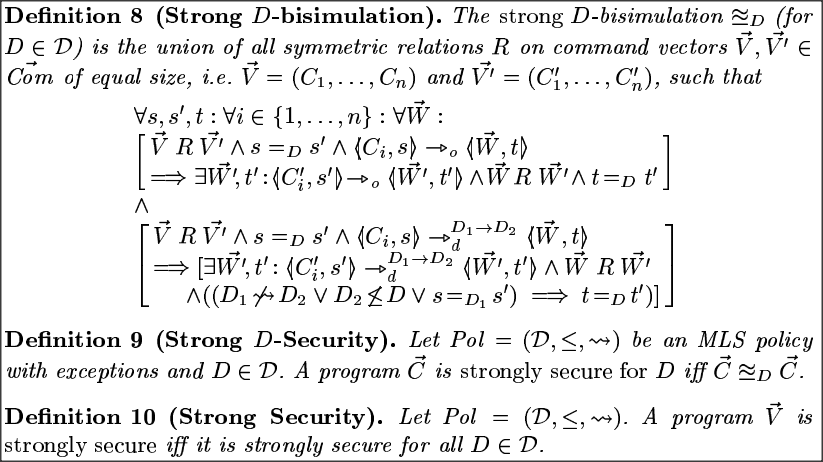
\includegraphics[scale=0.5]{pic/Mantel04.png}$
\begin{itemize}
  \item Adding the $\leadsto$ to an MLS policy changes where information flow is
  permitted, but does not affect visibility. An observer can still only see the
  values of variables at his clearance and below (according to $\leq$). In
  particular, the definition of D-equality remains unchanged;
  \item $\leq$ the information flow ordering;
  \item $\leadsto$ the information flow relation (declassification);
  \item $\rightarrow_o$ the ordinary transition;
  \item $\rightarrow^{D1 \rightarrow D2}_d$ the downgrading transition from
  $D_1$ to $D_2$;
  \item $s_1 =_D s_2$ iff $\forall var \in Var: dom(var) \leq D \Rightarrow
  s_1(var) = s_2(var)$;
  \item The definition means that: when the program performs a step, (1) if it's
  the ordinary transition $\rightarrow_o$, and the initial states $s$ and $s'$
  are D-equal, then their finals states $t$ and $t'$ are also D-equal;
  (2) else if it is the downgrading
  transition $\rightarrow^{D1 \rightarrow D2}_d$ from $D_1$ to $D_2$, and the
  initial states $s$ and $s'$ are D-equal, (2.1) if $D_1$ is not allowed to be
  downgraded to $D_2$ in policy, then this downgrading transition must not have
  any effect, (2.2) if $D_1$ is allowed to be downgraded to $D_2$, but $D_2$ is
  not a subset of $D$, it also must not have any effect, (2.3) if $D_1$ is
  allowed to be downgraded to $D_2$, and $D_2$ is a subset of $D$ and the
  initial states $s$ and $s'$ are D-equal, then we can conclude that their
  finals states $t$ and $t'$ are also D-equal;
  \item In this paper, $[Id := Id']$ is used as downgrading command;
  \begin{itemize}
    \item Code Locality: rather than localizing declassification in a program at
    the level of entire processes, they localize it at the level of individual commands;
    \item Level Locality: they restrict exceptions (downgrading) to certain
    parts of the security lattice;
  \end{itemize}
\end{itemize}






















\bibliographystyle{abbrv}
\newpage
\begin{thebibliography}{10}
\bibitem{Mantel:2004}
Controlled Declassification Based on Intransitive Noninterference, 2004.
\bibitem{Sabelfeld:2005}
Dimensions and Principles of Declassification, 2005.
\bibitem{Meyden:2009}
Architectural Refinement and Notions of Intransitive Noninterference, 2009.
\bibitem{Meyden:2007}
What, Indeed, Is Intransitive Noninterference?, 2007.


\bibitem{Chong:2004}
Security policy for downgrading, 2004.
\bibitem{Sabelfeld:2004}
A model for delimited information release, 2004.
\bibitem{Askarov:2007}
Gradual Release: Unifying Declassification, Encryption and Key Release Policies,
2007.
\bibitem{Banerjee:2007}
Expressive declassification policies and modular static enforcement, 2007.

\end{thebibliography}
 

\newpage
\setcounter{page}{1}

\end{document}


